The proposal consist on a possibilistic valid-time model. The representation and the querying are explained in the following subsections.

\subsection{Representation of ill-known valid-time intervals}
Valid time is usually represented as an interval. The interval has a starting and an ending points. An ill-known valid-time interval is an interval in witch one or both points are ill-known. 

\begin{definition}
A Possibilistic Valid-Time Period \textbf{PVP} is a possibilistic interval defined by means of two ill-known points, namely $\left[ X,\ Y \right]$
\begin{equation}
PVP = \left[X,\ Y \right] 
\end{equation}
$X$ and $Y$ are ill-known values in the set of the real numbers $\mathbb{R}$. The uncertainty about the values taken by $X$ and $Y$ are given by the possibility distributions $\pi_X$ and $\pi_Y$.
\end{definition}

The possibility distributions $\pi_X$ and $\pi_Y$ are given in the way of a triangular distribution, as explained in subsection \ref{subsec:fuzzy-numbers}. This representation allows overlapping (Fig. \ref{fig:pvp}).


\begin{figure}[h!]
  \centering
  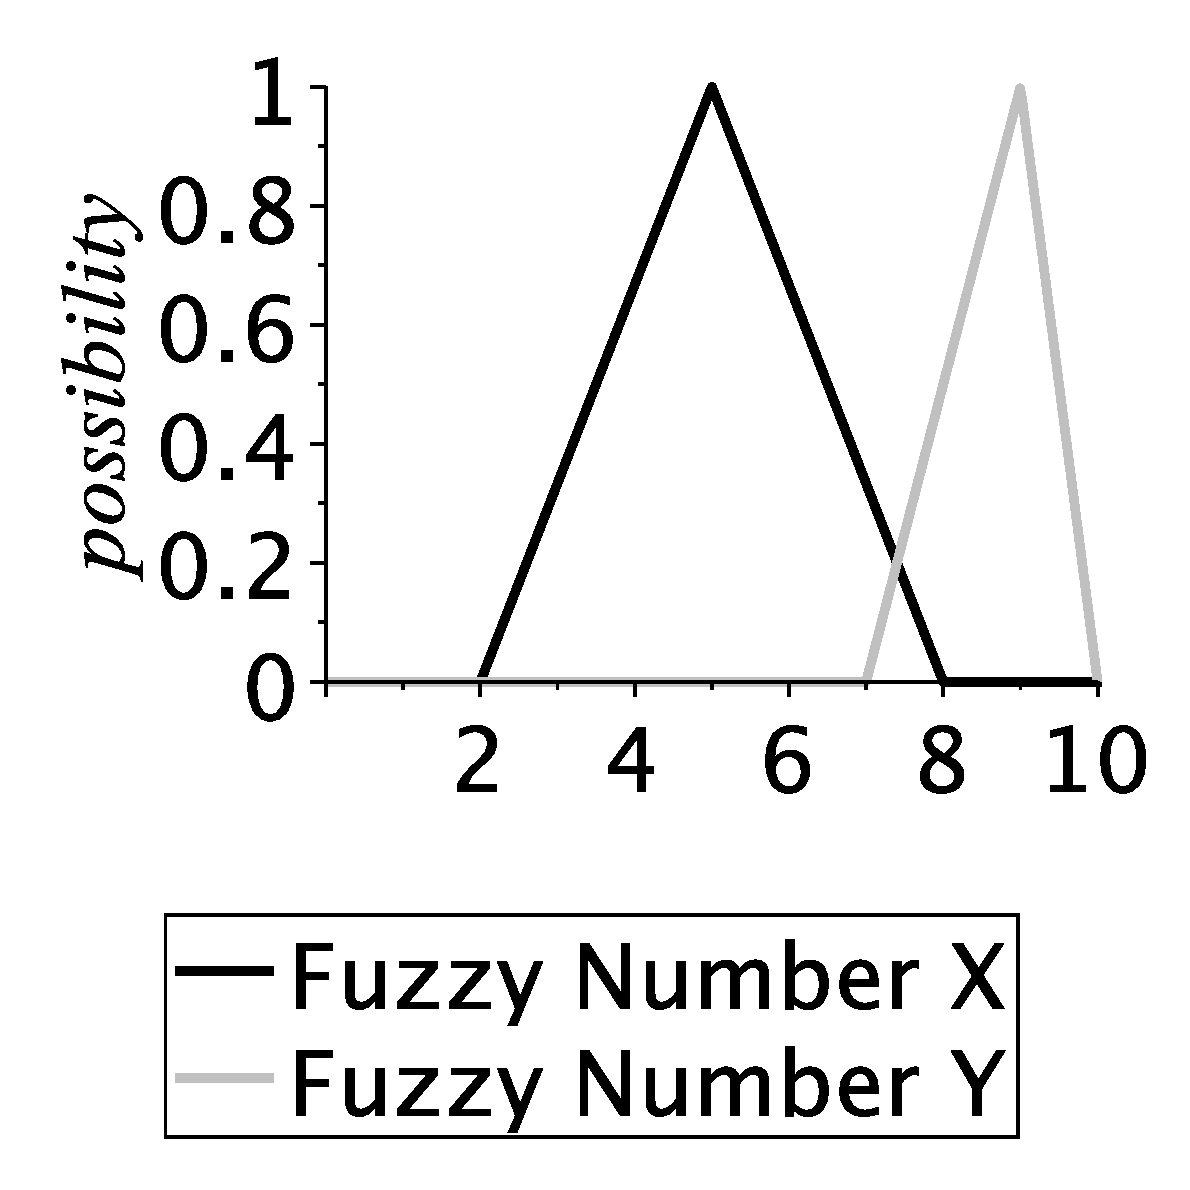
\includegraphics[scale=0.2]{graphs/2_triangular.eps}
  \caption{Two fuzzy numbers $X$ and $Y$ denoting a Possibilistic Valid-Time Period \emph{PVT}.}
  \label{fig:pvp}
\end{figure}

\subsection{Storage of valid-time intervals}
Each database row containing a \emph{PVP} stores it as two triangular possibility distributions. In our approach we propose the representation of that as proposed in the  fuzzy interface for relational databases \emph{FIRST}~\cite{Medina94gefred.a,Gal98}. In this representation it is also possible to represent not only fuzzy numbers but fuzzy constants (see table \ref{table:relational-representation-pvp}):

\begin{itemize}
\item
\emph{NULL}: This constant refers to a completely ignorance about the value. The possibility distribution for a given fuzzy number $X$ is not defined, therefore, any comparison between a fuzzy number and the \emph{NULL} constant always returns $0$.
\item
\emph{UNKNOWN}: The point has a value but it is unknown. The possibility distribution for a given fuzzy number $X$ is $\pi_X=1$
\item
\emph{UNDEFINED}: The point does not have a value. The possibility distribution for a given fuzzy number $X$ is $\pi_X=0$
\end{itemize}


\begin{table}
\caption{Relational representation for a Possibilistic Valid-Time Period.}
\centering
\begin{tabular}{c c c c c c}
\hline
Value & FT & F1 & F2 & F3  \\ \hline
UNKNOWN & 0 & NULL & NULL & NULL  \\ 
UNDEFINED & 1 & NULL & NULL & NULL  \\ 
NULL & 2 & NULL & NULL & NULL  \\ 
$\left[D,\ a,\ b \right]$ & 3 & $D$ & $D-a$ & $D+b$ \\ 
\hline
\end{tabular}
\label{table:relational-representation-pvp}
\end{table}

\subsection{Querying ill-known valid-time intervals}

\subsubsection{Query specification}

\subsubsection{Query evaluation}

\subsubsection{Ranking}